%    \begin{macro}
%    This macro is a helper macro to set the paper height and width
%    we also save the paper name in its own macro.
%    \begin{macrocode}
\gdef\setpapersize@cx#1#2#3{%
   \gdef\papername{#1}
   \setlength\paperheight{#2}
   \setlength\paperwidth{#3}
   % headheight is common to all so we set it here
   \setlength\headheight{12\p@}
}
%    \end{macrocode}
%    \end{macro}
%
%    \begin{macro}
%    \begin{macrocode}
\def\setparams@cx#1#2#3{%
    \def\X{11pt}\def\XX{11pt}
    % 11pt font set it as well
    \ifx\X\XX
          \@setfontsize\normalsize\@xipt{13.2}%
          \abovedisplayskip 13.2\p@ \@plus 3\p@ \@minus 3\p@
          \abovedisplayshortskip \z@ \@plus 3\p@
           \belowdisplayshortskip 6.6\p@ \@plus 3\p@ \@minus 3\p@
    \fi
    \setlength\headsep{#1}
    \setlength\footskip{#2}
    \setlength\topskip{#3}
    \setlength\maxdepth{0.5\topskip} % need to check
   }
%    \end{macrocode}
%    \end{macro}
%
%    We now set keys for all the paper sizes  
\cxset{
   a4paper/.code=\setpapersize@cx{a4paper}{297mm}{210mm},
   a5paper/.code=\setpapersize@cx{a5paper}{210mm}{148mm},
   b5paper/.code=\setpapersize@cx{b5paper}{250mm}{176mm},
   letterpaper/.code=\setpapersize@cx{letterpaper}{11n}{8.5in},
   legalpaper/.code=\setpapersize@cx{legalpaper}{14in}{8.5in},
   executivepaper/.code=\setpapersize@cx{executivepaper}{10.5in}{7.25in},
}
%    the classical dimesions were obtained from the Octavo class
%    we use mm or in depending on the type of paper standard
\cxset{foolscap/.code=\setpapersize@cx{foolscap}{171mm}{108mm},
          crown/.code=\setpapersize@cx{crown}{191mm}{127mm},
          post/.code=\setpapersize@cx{post}{194mm}{122mm},
          large post/.code=\setpapersize@cx{large post}{210mm}{137mm},
          demy/.code=\setpapersize@cx{demy}{222mm}{143mm},
          medium/.code=\setpapersize@cx{medium}{229mm}{146mm},
          royal/.code =  \setpapersize@cx{royal}{254mm}{159mm},
          superroyal/.code=\setpapersize@cx{superroyal}{267mm}{171mm}, 
          imperial/.code=  \setpapersize{imperial}{279mm}{191mm}}
%   Set the parameters that depend on font-sizes
\cxset{
         10pt/.code=\setparams@cx{6pt}{25pt}{10pt}\normalsize,
         11pt/.code=\setparams@cx{7pt}{27.5pt}{11pt},
         12pt/.code=\setparams@cx{8pt}{30pt}{12pt}
}%

%   we need to set a default size before we determine the
%   rest of the parameters.
\cxset{a4paper,11pt}

%    set a default top margin first
\setlength{\topmargin}{0.1\paperheight}
    \addtolength{\topmargin}{-\headheight}
    \addtolength{\topmargin}{-\headsep}
    \addtolength{\topmargin}{-1in}

\cxset{topmargin/.code=\setlength{\topmargin}{#1}}
\cxset{topmargin=0in}

%   \section{Calculation of textwidth}
%    The calculation of textwidth will depend on the strategy employed to calculate it.
% \begin{macro}{\textwidth}
%    Define the width of the text block to 0.7 of the page width, and make
%    calculations a little easier by adjusting the calculated width to a 
%    whole number of points.
%    \begin{macrocode}
\setlength{\textwidth}{0.7\paperwidth}
    \@settopoint\textwidth
%    \end{macrocode}
% \end{macro}
%
% \begin{macro}{\textheight}
%    The height of the text block itself is set to 0.7 times the page height. 
%    This amount is then adjusted to ensure that a whole number of lines makes 
%    up the text block, and does so exactly.
%    \begin{macrocode}
\setlength\@tempdima{0.7\paperheight}
%    \end{macrocode}
%    take away the first line, which is a bit shorter than the |\baselineskip|,
%    \begin{macrocode}
    \addtolength\@tempdima{-\topskip}
%    \end{macrocode}
%    this length may be very close, but just a little too small to accommodate 
%    one more line, so we add a small amount,
%    \begin{macrocode}
    \addtolength\@tempdima{5\p@}
%    \end{macrocode}
%    and calculate the number of lines in this length,
%    \begin{macrocode}
    \divide\@tempdima\baselineskip
    \@tempcnta=\@tempdima
%    \end{macrocode}
%    The correct textheight comes to the number of lines just calculated, 
%    multiplied by the height of text lines, |\baselineskip|, and with the 
%    addition of the |\topskip| we took away initially.
%    \begin{macrocode}
    \setlength\textheight{\@tempcnta\baselineskip}
    \addtolength\textheight{\topskip}
%    \end{macrocode}
% \end{macro}
%
% \subsubsection{Margin dimensions}
%     Now that we have set the size of the text block, the amount of space
%     available for margins is set as well. The remaining white space is divided
%     in a 1:2 ratio, hence the proportions between margins and text become 1:7:2.
%
% \begin{macro}{\evensidemargin}
% \begin{macro}{\oddsidemargin}
%    Since we are typesetting books, both even and odd side margins have to be
%    set.
%    \begin{macrocode}
\setlength{\evensidemargin}{0.2\paperwidth}
\addtolength{\evensidemargin}{-1in}
\setlength{\oddsidemargin}{0.1\paperwidth}
\addtolength{\oddsidemargin}{-1in}
%    \end{macrocode}

%    Define an innermargin to enable easy drawing of parameters
\newlength\innermargin
\newlength\lefttrim
\newlength\bottomtrim

%    The stockheight and stockwidth are used when the paper is to be trimmed
%    they default to the dimensions for paper width and paper height
\@ifundefined{stockheight}{\global\newlength\stockheight}{}
\@ifundefined{stockwidth}{\global\newlength\stockwidth}{}
\ifdim\stockheight=0pt\addtolength\stockheight{\paperheight}\fi
   \addtolength\stockheight{0mm}
%
\ifdim\stockwidth=0pt\addtolength\stockwidth{\paperwidth}\fi
   \addtolength\stockwidth{0mm}
%
%   We set all the trims to zero to start with.
\setlength\lefttrim{0mm}
\setlength\bottomtrim{0mm}
\setlength\trimtop{0mm}
\setlength\trimedge{0mm}
%
%   


%% This is a sidenote without the footnote mark
%\newcommand\marginnote[2][0pt]{%
% % \let\cite\@tufte@infootnote@cite%   use the in-sidenote \cite command
%  %\gdef\@tufte@citations{}%           clear out any old citations
%  \@tufte@margin@par%                 use parindent and parskip settings for marginal text
%  \marginpar{\hbox{}\vspace*{#1}\marginparfont@cx\marginparjustification@cx\vspace*{-1\baselineskip}\noindent #2}%
%  \@tufte@reset@par%                  use parindent and parskip settings for body text
%  %\@tufte@print@citations%            print any citations
%  %\let\cite\@tufte@normal@cite%       go back to using normal in-text \cite command
%}

% This macro has been adapted from the layouts package, it sets the units to be printed
% in the diagrams.
\newcommand{\printinunitsof@cx}[1]{%
  \def\l@yunitperpt{1.0}\def\l@yunits{pt}%
  \def\l@yta{#1}\def\l@ytb{pt}%
  \ifx \l@yta\l@ytb
    \def\l@yunitperpt{1.0}\def\l@yunits{pt}%
  \else
    \def\l@ytb{pc}%
    \ifx \l@yta\l@ytb
      \def\l@yunitperpt{0.083333}\def\l@yunits{pc}%
    \else
      \def\l@ytb{in}%
      \ifx \l@yta\l@ytb
        \def\l@yunitperpt{0.013837}\def\l@yunits{in}%
      \else
        \def\l@ytb{mm}%
        \ifx \l@yta\l@ytb
          \def\l@yunitperpt{0.351459}\def\l@yunits{mm}%
        \else
          \def\l@ytb{cm}%
          \ifx \l@yta\l@ytb
            \def\l@yunitperpt{0.0351459}\def\l@yunits{cm}%
          \else
            \def\l@ytb{bp}%
            \ifx \l@yta\l@ytb
              \def\l@yunitperpt{0.996264}\def\l@yunits{bp}%
            \else
              \def\l@ytb{dd}%
              \ifx \l@yta\l@ytb
                \def\l@yunitperpt{0.9345718}\def\l@yunits{dd}%
              \else
                \def\l@ytb{cc}%
                \ifx \l@yta\l@ytb
                  \def\l@yunitperpt{0.0778809}\def\l@yunits{cc}%
%                \else
%                  \def\l@ytb{PT}%
%                  \ifx \l@yta\l@ytb
%                    \def\l@yunitperpt{1.0}\def\l@yunits{PT}% gives problems with pgfmathparse
%                  \fi
                \fi
              \fi
            \fi
          \fi
        \fi
      \fi
    \fi
  \fi
}

% Define keys to set it
\cxset{geometry units/.code=\printinunitsof@cx{#1}}
\cxset{geometry units=pt}

% #1 value in pts
% default in mm sorry USA.
% rounding in 1 decimal place
\def\convert@cx#1{%
   \pgfmathparse{#1*\l@yunitperpt}
   %\pgfmathround{\pgfmathresult}
   \pgfmathresult\thinspace\l@yunits
}

% Layout related macros to go to separate style file
\def\aspectratio{\pgfmathparse{\paperheight/\paperwidth} \pgfmathresult}



\def\alignedge{%
  \checkoddpage%
  \parindent0pt%
%   \ifoddpage \global\setlength\innermargin{\oddsidemargin}
%          \else \global\setlength\innermargin{\evensidemargin}
%      \fi%
%   \if@twoside\setlength\innermargin{\dimexpr(\evensidemargin-\marginparsep)}%
%             \else\let\innermargin\oddsidemargin\fi
   \ifoddpage 
      \innermargin\oddsidemargin
      \def\innermarginname{oddsidemargin}%
     \else
        \innermargin\evensidemargin
        \def\innermarginname{evensidename}%
  \fi
  }

\alignedge


% Set to true to draw an oddside page. Initially set to false.
\newcommand\layoutscale@cx{0.35}

\newif\ifoddpagelayout@cx
   \oddpagelayout@cxtrue

% Set true to draw marginpars on a page
\newif\ifdrawmarginpars
   \drawmarginparstrue

% This draws a two page spread
\newlength\bindingcorrection
\newlength\oneninth
\newlength\sixninths
\setlength\oneninth{\dimexpr(\paperwidth/9)}
\setlength\sixninths{\dimexpr(\paperwidth*6/9)}
\let\trytextwidth\sixninths


\newcommand{\alphabet}{abcdefghijklmnopqrstuvwxyz}%82



\newcommand\charactersperline{%
  \settowidth{\@tempdima}{\alphabet}
  \pgfmathparse{\textwidth/\@tempdima*26}
  \pgfmathresult
}

\newcommand\alphabetsperline{
  \settowidth{\@tempdima}{\alphabet}
  \pgfmathparse{\textwidth/\@tempdima}
  \pgfmathresult
}

\newcommand\alphabetlength{%
  \settowidth{\@tempdima}{\alphabet}
 \the\@tempdima
}

% We need to use the fp package to calculate the ratios, as PGF has problems with large 
% dimensions
\newcommand\textarearatio{%
    \FPmul{\result}{\strip@pt\textwidth}{\strip@pt\textheight}
    \FPmul{\resulti}{\strip@pt\paperwidth}{\strip@pt\paperheight}
    \FPdiv{\resultii}{\result}{\resulti}
    \resultii
}

% Calculate the ratio textheight/paperheight
\newcommand\textheightratio{%
    \FPdiv{\result}{\strip@pt\textheight}{\strip@pt\paperheight}
    \FPround{\result}{\result}{2}
    \result
}

\newlength\margintop

\newcommand\thetop{%
   \pgfmathparse{1in+\topmargin+\headheight+\headsep}
   \pgfmathsetlength{\margintop}{\pgfmathresult}
}

\thetop

\newlength\marginbottom
\newcommand\thebottom{%
   \pgfmathparse{\stockheight-(1in+\topmargin+\headheight+\headsep+\textheight)}
    \pgfmathsetlength{\marginbottom}{\pgfmathresult}
  }
\thebottom

\newcommand\verticalmarginratio{%
\pgfmathparse{(\paperheight-(1in+\topmargin+\headheight+\headsep+\textheight))/  (\paperheight-(1in+\topmargin+\headheight+\headsep+\textheight))}
\pgfmathresult
}

\newcommand\horizontalmarginratio{%
\pgfmathparse{(\paperwidth-\textwidth-\oddsidemargin)/(1in+\oddsidemargin)}
\pgfmathresult
}

\newcommand\numbertextlines{%
% baselineskip to be corrected
   \pgfmathparse{(\textheight-\topskip)/(12)-1}\pgfmathresult
}

\cxset{geometry units=mm}

\def\printgeometryvalues{%
   \noindent
   \begin{tabular}{ll}
   papername & \papername\\
   paperwidth & \convert@cx{\paperwidth}\\
   paperheight & \convert@cx{\paperheight}\\
   voffset & \convert@cx{\voffset}\\
   hoffset & \convert@cx{\hoffset}\\
   thetextheight & \convert@cx{\textheight}\\
   thetextwidth  & \convert@cx{\textwidth}\\
   Top margin   &  \thetop\convert@cx{\the\margintop}\\  % need to correct
   Bottom margin & \thebottom\\
   thetopmargin & \convert@cx{\topmargin}\\
   theheadheight & \convert@cx{\headheight}\\
   theheadsep & \convert@cx{\headsep}\\
   theoddsidemargin & \convert@cx{\oddsidemargin}\\
   theevensidemargin & \convert@cx{\evensidemargin}\\
   themarginparsep& \convert@cx{\marginparsep}\\
   themarginparwidth& \convert@cx{\marginparwidth}\\
   themarginpush& \convert@cx{\marginparpush}\\
   thevoffset& \convert@cx{\voffset}\\
   thefootskip& \convert@cx{\footskip}\\
   aspect ratio \aspectratio\\
   twoside&  \if@twoside true\else false\fi\\
   reversemarginpar& \if@mparswitch true \else false\fi\\
  \end{tabular}
 }

\def\readability{%
\begin{tabular}{ll}
Characters per line &\charactersperline\\
Alphabets per line &\alphabetsperline\\
Alphabet length &\alphabetlength\\
Baselineskip & \the\baselineskip\\
Number of text lines &\numbertextlines\\
Text area ratio & \textarearatio\\
Text/page height ratio & \textheightratio\\
Vertical margin ratio &\verticalmarginratio\\
Horizontal margin ratio &1:\horizontalmarginratio\\
\end{tabular}}


% Note with new geometry paper has to be defined in preamble
% I do not feel very confident of this
% Don't understand it fully how is working
 %\@twosidefalse \@mparswitchfalse % one side option
%\cxset{geometry oxford/.code={
%\newgeometry{left=74.8mm,top=27.4mm,headsep=2\baselineskip,%
%marginparsep=8.2mm,marginparwidth=49.4mm,textheight=49\baselineskip,headheight=\baselineskip}
%\@twosidefalse \@mparswitchfalse % one side option
%\reversemarginpar
%}}
% \@mparswitchfalse
%\cxset{geometry textwidth/.store in=\textwidth@cx,
%          geometry textheight/.store in=\textheight@cx,
%          geometry tufte/.code={
%             \newgeometry{a4paper,left=24.8mm,top=27.4mm,headsep=2\baselineskip,%
%             textwidth=107mm,marginparsep=8.2mm,marginparwidth=49.4mm,%
%             textheight=\textheight@cx\baselineskip,headheight=\baselineskip}
%            \@twosidefalse \@mparswitchfalse % one side option
%           %\reversemarginpar
%    }
%}
%
%
%\cxset{marginpar push/.store in=\marginparpush@cx,
%          marginpar font/.store in=\marginparfont@cx,
%          marginpar justification/.is choice,
%          marginpar justification/justifying/.code=\gdef\marginparjustification@cx{\justifying},
%          marginpar justification/raggedright/.code=\gdef\marginparjustification@cx{\raggedright},
%          marginpar justification/RaggedRight/.code=\gdef\marginparjustification@cx{\RaggedRight},
%          marginpar justification/RaggedLeft/.code=\gdef\marginparjustification@cx{\RaggedLeft},
% }
%%\cxset{marginpar push=10pt,
%%          marginpar font=\normalfont\footnotesize\sffamily,
%%          marginpar justification=RaggedLeft}
%%
%%
%%\cxset{style13, geometry textheight=47,
%%          %geometry tufte,
%%          watermark text=SAMPLE TUFTE VARIANT,
%%          watermark text color=thered,
%%          header style=samplepage}
%%%%%%%%%%%%%%%%%%%%
\chapter{Geometry and Page Dimensions}
\parindent1.5em

\section{Introduction}

Setting up the page geometry, is normally done by the class or if adjustments need to be made, most authors will use the package geometry. If you need to view the geometry and the values of the document layout you can use the pkg{layouts}. This package offers a set of convenience key values for setting up geometry in order to enable authors to have a comprehensive style sheet.

\section{How to set geometry via this package}

To set the geometry page of the whole document, set the keys in the preamble. To change the page geometry anywhere in the document use the appropriate style or keys where you want the page geometry to change.
Note that the paper zize can only be defined in the preamble. The package is more useful when loaded with predefined styles.

\begin{tcolorbox}
\begin{lstlisting}
\cxset{page geometry=medieval}
\end{lstlisting}
\end{tcolorbox}

In most instances you will want to load the geometry at the style sheet.


\section{Viewing the page geometry}

The package offers a number of keys to set documents either document wide or locally to change page 
parameters or to view the frames. this is very similar to what the layouts and geometry packages offer. We do
however use TikZ for these diagrams.

To incorporate a layouts diagram we offer two macros \cs{printlayout} and \cs{printlayoutvalues}. Both have associated styling keys.
\medskip

\section{Technical discussion}
\subsection{The LaTeX standard classes}

LaTeX has pre-build layouts that are based on two variables. The \textit{paper size} and the \textit{font size}. Appropriate values are calculated in the class.

\subsection{Other common classes}

The more generic classes such as memoir and koma-script offer extensive customization and calculation of page parameters. They all use the basic laTeX page terminology which they supplement for additional parameters.

The octavo class offers a set of paper sizes suited for classical layouts printed on classical sizes such as the octavo. Classes such as the tufte-book offer a fixed design and no special commands for parameter manipulation.
\subsection{Paper sizes}
Most people using LaTeX, will print on either a4paper or letterpaper sizes. If you going to bind the work it might be necessary to trip the paper a little bit during binding to make sure that the top and side of the book are not ragged. This is normally called the \textit{trim}. If the document is to be printed by a publishing house this might be done by the printer which will use a different size \textit{stock size}. They might also allow for two additional dimensions called the spinemargin or the foremargin.

\subsection{The page dimensions}

The page dimensions are shown in figure 1. We tried to cater for the common terminology of all the classes.

\subsection{Texwidth}

The width of the text can only be determined based on the designer's strategy and is inexorably tied also to
the textheight. For example in classical page design, the designer tried to get the textwidth to be the same size like
the page width, thus giving an almost squarish look. Another strategy is the 6-9 strategy, where the paper is divided into a grid of 9 equal blocks and the textwidth occupies the 6. 

\subsection{Readability considerations}

An average line that is longer than 40 to 70 characters long -- inluding spaces, is difficult to read. This is generally applicable to European languages and might be different for other languages. In addition the average number of words in one line should also be considered. For the German language Willi Egger (2004) recommends a line consisting of 8 to 12 words as optimal. If this strategy is adopted one can determine the line length based on the number of letters.

The characters per line for this document is \charactersperline

\subsubsection{Simple strategy}
However, despite most of the above typesetting strategies many an author just want to take an approach, where they specify the margins and want to get what they need for example a spine margin of 1cm and an edge margin of 1.5cm. This is also important for screen dimensions.

\begin{lstlisting}
\cxset{
    margin inner= 1in
    margin outer= 2in
    margin top=1in
    margin bottom=2in
}
\end{lstlisting}

If all four margins are specified, the typesetting area can be positioned on the paper block. Life is not this easy though.



\subsection{Textheight}

When using \cs{flushbottom} LaTeX expects that the \cs{textheight} is such that a number of textlines in the body font will fit exactly into the height. If not, it issues an underfull vbox's message. LaTeX calculates these parameters when loading the class .clo files.
 



\section{Allowing for trims}
\newpage

%\topmargin0pt
\cxset{geometry units=in}
\reversemarginparfalse

\def\drawlayout{%
\checkoddpage
\alignedge
\tikzset{dim/.style = {>= latex,color=black}}
\begin{tikzpicture}[scale=0.35,font={\scriptsize\rmfamily},line width=.8pt,
       every node={color=black}]
% draw stockwidth and stockheight
\draw [color=gray] (0,0) rectangle ++(\stockwidth,\stockheight);


% draw the paper 
\draw [color=NavyBlue,dashed]  (0+\lefttrim,\stockheight-\trimtop) rectangle ++ (\stockwidth-\lefttrim-\trimedge,-\stockheight+\trimtop+\bottomtrim);
% dimensions one more try
%\cxset{geometry units=mm}
% paper width dimensions, better to change to a macro
% tol is the distance to dimension

% paper width
\edef\tol{-2.5\baselineskip}
\coordinate (A) at (0+\lefttrim,\tol);
\coordinate (B) at (\stockwidth-\trimedge,\tol);
\coordinate (C) at (0.5\stockwidth,\tol);
\draw[dim, |<->|] (A) -- (B); 
\node at (C) [yshift=0.5\baselineskip)]{paper width = \convert@cx{\paperwidth}};

% stockwidth
\edef\tol{-5\baselineskip}
\coordinate (BD) at (0,\tol);
\coordinate (BD2) at (\stockwidth,-5\baselineskip);
\draw[dim, |<->|] (BD) -- (BD2); 
\node at (BD)[yshift=0.5\baselineskip,xshift=0.25*\stockwidth]{stockwidth=\convert@cx{\stockwidth}} ;

% top dimension at left
\coordinate (H1) at (-5mm,\stockheight);
\coordinate (H2) at (-5mm,\stockheight-1in-\topmargin-\headsep-\headheight);
\draw [dim,|<->|] (H1) -- (H2);
\node[left,text width=1.5cm, text ragged left] at (-5mm,\stockheight-0.5*\margintop){top\\ \convert@cx{\the\margintop}};

% bottom dimension at left
\coordinate (H3) at (-5mm,0);
\coordinate (H4) at (-5mm,\marginbottom);
\draw [dim,|<->|] (H3) -- (H4);
\node[left] at (-5mm,0.5*\marginbottom){\convert@cx{\the\marginbottom}};

% textheight at left
\draw[dim,<->]  (-5mm, \marginbottom) -- ++ (0,\textheight);
\node[left,text width=1.5cm,text ragged left] at (-5mm,\marginbottom+0.5\textheight){textheight \convert@cx{\the\textheight}};


% trimedge
\coordinate (D) at (\stockwidth-4\trimedge, 0.10\textheight);
\coordinate (E) at (\stockwidth,0.10\textheight);
\draw [dim,->|] (D) -- ++(3\trimedge,0);
\draw [dim,|<-|] (E) -- ++(3\trimedge,0) node at ++(0,0) [right,text width=2cm,color=black] {trim edge \convert@cx{\the\trimedge}};

% toptrim
%\ifdim\trimtop>0pt
  \coordinate (F) at (0.9\stockwidth, \stockheight-\trimtop-8mm);
  \coordinate (G) at (0.9\stockwidth, \stockheight-\trimtop);
  \coordinate (H) at (0.9\stockwidth,\stockheight);
  \draw (F)[dim,->|] -- (G);
  \draw (H) -- ++ (0,8mm) -- ++ (5mm,0)[|<-|,>=latex] 
          node [right] at ++ (0,0) {top trim =  \convert@cx{\the\trimtop}};
%\fi

% 1in offsets
\draw[dashed,color=gray] (1in,0) -- (1in,\stockheight);
\draw[dashed,color=gray] (0in,\stockheight-1in)-- ++ (\stockwidth,0);

% oddsidemargin/evensidemargin
% draw dimension and name based on even or odd page
\draw[dim,|<->|] (0,0.1\textheight) -- ++(1in+\innermargin,0) node[right] at ++ (2ex,0) [text width=2cm,color=red] {\innermarginname\  \convert@cx{\the\innermargin}};

% HEADER
\coordinate (I) at (1in-\lefttrim+\innermargin,\stockheight-1in-\headheight-\topmargin+\trimtop);
\draw (I) rectangle ++ (\textwidth,\headheight);

%\draw[dim,<->] (1.5in\tol,\stockheight) -- ++(0,-1in) node[above right] at ++ (0,0.2in) {1in + yoffset};

% add in inch 
\draw [dim,|-] (\stockwidth+3ex,\stockheight-\trimtop)
      -- ++(0,-1in) node [right] at ++(2ex,0.5in) {offset=\convert@cx{1in}};

%   add topmargin dimension
\draw [dim,|-|] (\stockwidth+3ex,\stockheight-1in+\trimtop)
      -- ++(0,-\topmargin) node [right] at ++(2ex,0.5\topmargin) {topmargin=\convert@cx{\topmargin}};

%  add headheight dimension
\draw [dim,-|] (\stockwidth+3ex,\stockheight-1in+\trimtop-\topmargin)
        -- ++(0,-\headheight) node [right] at ++(2ex,0.5\headheight) {headheight=\convert@cx{\the\headheight}};

%   add headsep dimension
\draw [dim,|-] (\stockwidth+3ex,\stockheight-1in+\trimtop-\headsep-\headheight-\topmargin)
          -- ++(0,\headsep) node [below right] at ++(2ex,0){headsep = \convert@cx{\the\headsep}};
% footskip dimension
\draw [dim,|-|] (\stockwidth+3ex,\stockheight-1in+\trimtop-\headsep-\headheight-\topmargin-\textheight) -- ++(0,-\footskip) node [right] at ++(2ex,0.5\footskip){footskip=\convert@cx{\the\footskip}};


% textarea
\coordinate (J) at (1in-\lefttrim+\innermargin,\stockheight-1in+\trimtop-\headheight-\topmargin-\headsep-\textheight);
\draw[fill=lightgray!50] (J) rectangle ++ (\textwidth,\textheight);

\draw[dim,<->|] (1in-\lefttrim+\innermargin,0.75\textheight) -- ++(\textwidth, 0)  node at ++(-0.5\textwidth,0.5\baselineskip) {textwidth} node at ++ (-0.5\textwidth,-\baselineskip) {\convert@cx{\the\textwidth}};

% draw grid
\draw[xstep=(\paperwidth-\trimedge)/9, ystep=(\stockheight-\trimtop)/9,color=gray,dotted]  (0,0) grid (\paperwidth,\paperheight); 
%%   add textheight dimension
%\draw [dim,-] (\stockwidth+3ex,\stockheight-1in+\trimtop-\headsep-\headheight-\topmargin) -- ++(0,-\textheight) node [right] at ++(2ex,0.5\textheight){textheight=\convert@cx{\the\textheight}};

% footer
\coordinate (I) at (1in-\lefttrim+\innermargin,  \stockheight-1in+\trimtop-\headheight-\topmargin-\headsep-\textheight-\footskip);
\draw (I) rectangle ++ (\textwidth,\headheight);


% marginpar
\def\leftmarginpar{%
    \draw [fill=Linen,opacity=0.7] (1in+\innermargin+\textwidth+\marginparsep,   \stockheight-1in+\trimtop-\topmargin-\headsep-\headheight ) rectangle ++(\marginparwidth,-\textheight);
 \draw [dim,|<->|] (1in-\lefttrim+\textwidth+\innermargin+\marginparsep+\marginparwidth,0.75\textheight) -- ++ (-\marginparwidth,0) node at ++(0.5\marginparwidth,0.5\baselineskip) {marginpar} node at ++(0.5\marginparwidth,-\baselineskip){\convert@cx{\the\marginparwidth}};
}

\def\rightmarginpar{%
 \draw [color=red] (1in+\innermargin-\marginparsep,\stockheight-1in+\trimtop-\topmargin-\headsep-\headheight ) rectangle ++(-\marginparwidth,-\textheight);
     \draw [dim,|<->|] (1in-\lefttrim+\innermargin-\marginparsep-\marginparwidth,0.75\textheight) -- ++ (\marginparwidth,0) node at ++(-0.5\marginparwidth,0.5\baselineskip) {marginpar} node at ++(-0.5\marginparwidth,-\baselineskip){\convert@cx{\the\marginparwidth}};
}

\ifdrawmarginpars
  \checkoddpage
  \alignedge
    \if@twoside
         \ifoddpage
            \leftmarginpar
         \else
            \rightmarginpar
        \fi
   \else
  % one side paper
        \leftmarginpar
    \fi
\fi

\ifoddpage
     \draw [color=blue]  (\stockwidth,0) -- (0, \stockheight);
  \else
    \draw [color=blue] (0,0) -- (\stockwidth,\stockheight);
\fi  
\end{tikzpicture}
}

\drawlayout
 
\clearpage

\drawlayout



\def\spread{%
\begin{tikzpicture}[scale=0.25]
% draw the two pages
\setlength\bindingcorrection{60pt}
\draw[xstep=\paperwidth/9,ystep=\paperheight/9, line width=1.2pt] (0,0) rectangle (\paperwidth,\paperheight)  (\paperwidth+\bindingcorrection,0) rectangle ++(\paperwidth,\paperheight);

% draw the binding correction
\draw[fill=gray, draw] (\paperwidth,0)  rectangle ++(\bindingcorrection,\paperheight);

\draw[xstep=(\paperwidth)/9, ystep=(\stockheight)/9,color=gray,]  (0,0) grid (\paperwidth,\paperheight);

\draw[xstep=(\paperwidth)/9, ystep=(\stockheight)/9,color=gray]  (\paperwidth+\bindingcorrection,0) grid ++(\paperwidth,\paperheight);

% add type areas

\draw[fill=gray] (0+2\paperwidth/9,\paperheight/9) rectangle ++ (\trytextwidth,7pt+\paperheight-2\paperheight/9);

\draw[fill=gray] (\paperwidth+\paperwidth/9+\bindingcorrection,\paperheight/9) rectangle ++ (\trytextwidth,7pt+\paperheight-2\paperheight/9);

\ifdim\bindingcorrection>0pt
\draw[color=white,font={\sffamily\bfseries}] node at (\paperwidth+0.5\bindingcorrection, 0.5\paperheight)[rotate=90,inner sep=0pt,outer sep=0pt] {BINDING CORRECTION};\fi

\node [color=white,font={\sffamily\bfseries}] at (0.5\paperwidth,0.5\paperheight)  {LEFT PAGE};
\node [color=white,font={\sffamily\bfseries}] at (1.5\paperwidth+\bindingcorrection,0.5\paperheight){RIGHT PAGE};
\end{tikzpicture}
}

\spread
\bigskip

%\printgeometryvalues{}
\readability
% end of two page spread
\printgeometryvalues

\clearpage



\subsection{Headers and footers}
A page may have two additional items, and usually has at least one of these. They are the
running header and running footer. If the page has a folio then it is located either in the
header or in the footer. The word ‘in’ is used rather lightly here as the folio may not be
actually in the header or footer but is always located at some constant relative position. A
common position for the folio is towards the fore-edge of the page, either in the header or
the footer. This makes it easy to spot when thumbing through the book. It may be placed
at the center of the footer, but unless you want to really annoy the reader do not place it
near the spine.

Often a page header contains the current chapter title, with perhaps a section title on
the opposite header, as aids to the reader in navigating around the book. Some books put
the book title into one of the headers, usually the verso one, but I see little point in that as
presumably the reader knows which particular book he is reading, and the space would
be better used providing more useful signposts.

\section{Floating parameters}



%%\end{document}
%\lipsum[1-4]\marginnote[1pt]{\lorem
%    \lorem}
%
%\lipsum[1-2]

%% Stick the caption in the head might as well place the first picture also
\def\asidecaption{\parbox{4.2cm}{{\bfseries Image \thefigure}\par\lorem}%
  % \addtocontents{lof}{This is image 8}
}
\def\ps@caption{%
     \let\@oddfoot\@empty\let\@evenfoot\@empty%
    \def\@evenhead{%
        \begin{picture}(0,0)%
           \put(-150,-80){\asidecaption\par}%
            \stepcounter{figure}
           \put(-150,-370){\asidecaption}%
        \end{picture}%
      }%
    \let\@oddhead\@evenhead%
    \let\@mkboth\@gobbletwo%
    \let\chaptermark\@gobble%
    \let\sectionmark\@gobble%
 }

\def\ps@bigpicture{%
    \setlength\headheight{19cm}%
    \let\@oddfoot\@empty\let\@evenfoot\@empty%
    \def\@evenhead{%
         \begin{picture}(0,0)%
          \put(-149,0){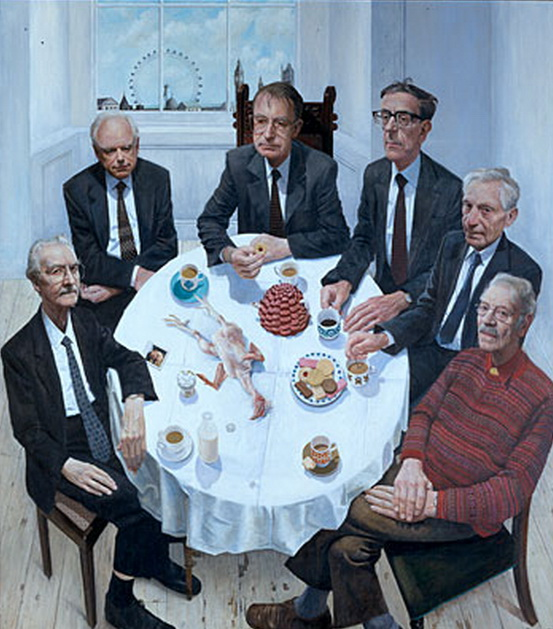
\includegraphics[width=\dimexpr(\textwidth+150pt)]{stuartpearson}}%
         \end{picture}%
      }%
    \let\@oddhead\@evenhead%
    \let\@mkboth\@gobbletwo%
    \let\chaptermark\@gobble%
    \let\sectionmark\@gobble%
 }



\def\doubletakeimage{%
  \renewcommand{\topfraction}{.95}  % ensure seecond image will not float away
  \begin{figure}[t]
    \thispagestyle{caption}
    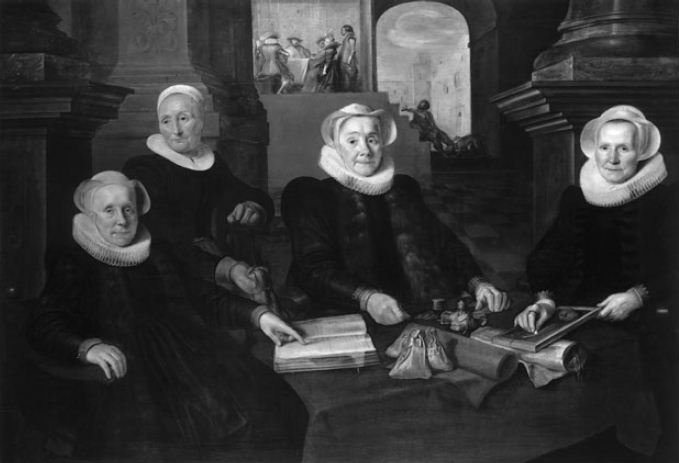
\includegraphics[width=\textwidth]{matron}%
  \end{figure}

  \begin{figure}[tp]
   \hspace*{-\marginparwidth}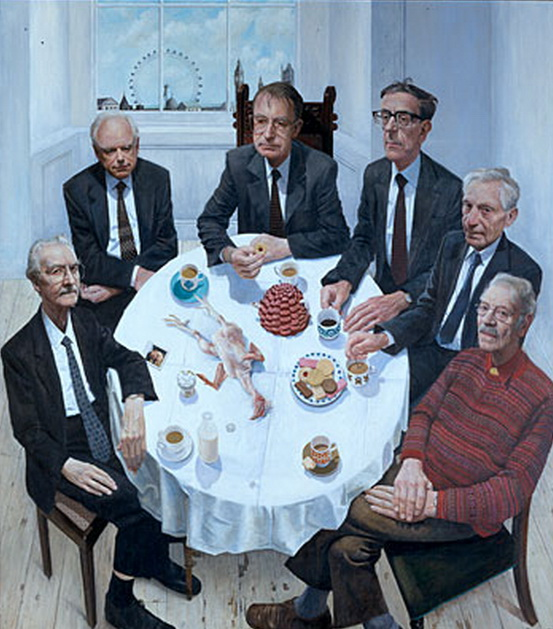
\includegraphics[height=0.9\textheight]{stuartpearson}
 \end{figure}
}




\lipsum[1-4]
\begin{figure}[htp]
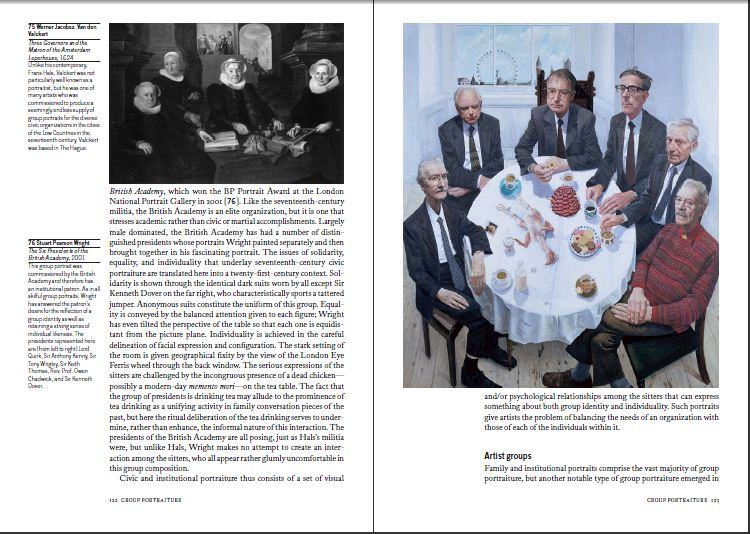
\includegraphics[width=0.98\textwidth]{captionspecial}
\centering
\caption{Figure from \textit{Oxford History of Art, Portraiture}, Shearer West, Oxford University Press, 2004. The figures are numbered consecutively and the text in the List of Illustrations have different formatting.}
\end{figure}

\doubletakeimage


\restoregeometry

%% RESET EVERYTHING AT END OF CHAPTER
\addtocounter{chapter}{-2}

\@toctrue\@specialtrue
\end{document}